\chapter{Dźwięk, próbkowanie i wysokość}\label{rozdz:dzwiek}

\section{Od drgania do liczb}

Struna gitary drga, pudło przekazuje drgania powietrzu, mikrofon zamienia zmiany ciśnienia na napięcie,
a komputer zapisuje to napięcie jako ciąg liczb. Cała wiedza, jaką model ma o nagraniu, to ten ciąg liczb.
Żeby ją wydobyć, trzeba najpierw zrozumieć dwie rzeczy: czym jest wysokość dźwięku
i co się traci przy zamianie fali ciągłej na liczby.

Po tym rozdziale umiesz: (i)~policzyć częstotliwość dowolnej nuty z jej numeru MIDI, (ii)~zmierzyć odstęp
dwóch dźwięków w centach, (iii)~uzasadnić, dlaczego model pracuje przy $11\,025\Hz$ i nie widzi wyższych częstotliwości
niż $5512{,}5\Hz$, (iv)~policzyć, ile klatek ma nagranie.

\section{Sinusoida}

\haslo{częstotliwość}
\begin{definicja}[Sinusoida, częstotliwość, okres]\label{def:sinusoida}
\emph{Sinusoidą} nazywamy sygnał $x(t)=A\sin(2\pi f t+\varphi)$ zmiennej $t$ (czas w sekundach). Liczba $A\ge0$ to
\emph{amplituda}, $f$ to \emph{częstotliwość} w hercach ($1\Hz$ = jeden pełny obieg na sekundę), a $\varphi$ to
\emph{faza}. Sygnał powtarza się co $T=1/f$ sekund; $T$ nazywamy \emph{okresem}.
\end{definicja}

\begin{przyklad}\label{prz:a4}
Strojowe A (nuta A4) ma $f=440\Hz$, więc okres $T=1/440\approx2{,}27\ms$. W ciągu jednej sekundy
powietrze wykonuje $440$ pełnych drgań. Dla sinusoidy $x(t)=0{,}5\sin(2\pi\cdot440\,t)$ największe wychylenie
wynosi $0{,}5$ i powtarza się co $2{,}27\ms$.
\end{przyklad}

\begin{intuicja}
Sinusoida to ruch punktu po okręgu oglądany z boku: faza mówi, skąd zaczynamy, a częstotliwość, ile obiegów
robimy na sekundę. Każdy dźwięk muzyczny to suma sinusoid; w rozdziale~\ref{rozdz:alikwoty} zobaczymy, że nuta gitary to
sinusoida $f_0$ i jej całkowite wielokrotności.
\end{intuicja}

\section{Próbkowanie}

Komputer nie widzi sygnału w każdej chwili, tylko co ułamek sekundy.

\haslo{próbkowanie}
\begin{definicja}[Próbkowanie]\label{def:probkowanie}
Dla sygnału $x(t)$ i \emph{częstotliwości próbkowania} $f_s$ ciąg próbek to $x[n]=x(n/f_s)$ dla $n=0,1,2,\dots$.
Jedna próbka to jedna liczba; nagranie trwające $\tau$ sekund ma $N=\tau f_s$ próbek.
\end{definicja}

\begin{przyklad}\label{prz:probkowanie}
Płyta CD ma $f_s=44\,100\Hz$, więc minuta dźwięku to $60\cdot 44\,100=2\,646\,000$ liczb. Model Gen~6 zmienia
próbkowanie nagrania na $f_s=11\,025\Hz$ (dokładnie ćwierć 44\,100): 6 sekund to $N=66\,150$ próbek.
\end{przyklad}

Pojawia się pytanie: ile informacji tracimy? Okazuje się, że dwie różne sinusoidy mogą dać \emph{identyczne} próbki.

\begin{twierdzenie}[Aliasing]\label{tw:aliasing}
Niech $f_s>0$. Dla każdej liczby całkowitej $k$ sinusoidy o częstotliwościach $f$ i $f+kf_s$ mają te same próbki.
Ponadto sinusoidy $\sin(2\pi f t)$ i $-\sin(2\pi (f_s-f)t)$ mają te same próbki. W szczególności sygnały
o częstotliwościach powyżej $f_s/2$ są nierozróżnialne od sygnałów o częstotliwościach poniżej $f_s/2$.
\end{twierdzenie}
\begin{pomyslDowodu}
Wstawiamy $t=n/f_s$ i korzystamy z tego, że sinus ma okres $2\pi$, a $n$ jest całkowite.
\end{pomyslDowodu}
\begin{proof}
Dla $t=n/f_s$ i $k\in\mathbb Z$:
\begin{align*}
\sin\!\big(2\pi (f+kf_s)\tfrac{n}{f_s}\big)
  &= \sin\!\big(2\pi f\tfrac{n}{f_s}+2\pi kn\big) && \pow{(rozdzielność)}\\
  &= \sin\!\big(2\pi f\tfrac{n}{f_s}\big) && \pow{($kn\in\mathbb Z$, okres $2\pi$)}
\end{align*}
To jest pierwsza część. Dla drugiej częstotliwość $f_s-f$ daje
\begin{align*}
\sin\!\big(2\pi (f_s-f)\tfrac{n}{f_s}\big)
  &= \sin\!\big(2\pi n-2\pi f\tfrac{n}{f_s}\big) && \pow{(wymnożenie)}\\
  &= -\sin\!\big(2\pi f\tfrac{n}{f_s}\big) && \pow{(nieparzystość sinusa, okres)}
\end{align*}
Zatem $-\sin(2\pi(f_s-f)n/f_s)=\sin(2\pi fn/f_s)$. Skoro każda częstotliwość większa niż $f_s/2$ ma postać
$f_s-f$ z $f<f_s/2$ (po odjęciu odpowiedniej wielokrotności $f_s$), jej próbki zgadzają się z próbkami
niższej częstotliwości. To kończy dowód.
\end{proof}

W zwykłym języku: przy próbkowaniu $f_s$ da się odróżnić tylko częstotliwości z przedziału $[0,f_s/2]$; wyższe
„zawijają się” w niższe (rys.~\ref{rys:probkowanie}b). Liczbę $f_s/2$ nazywamy \emph{częstotliwością Nyquista}.

\begin{figure*}[ht]
\centering
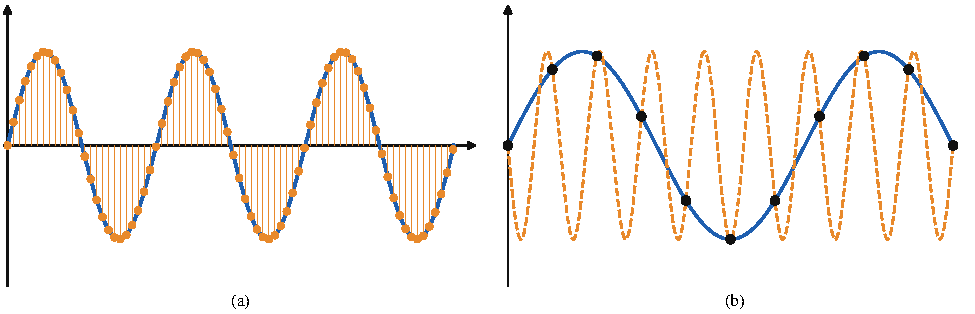
\includegraphics[width=\linewidth]{figures/probkowanie.pdf}
\caption{(a) Sinusoida $440\Hz$ (niebieska) i jej próbki przy $f_s=11\,025\Hz$ (pomarańczowe kropki): około
25 próbek na okres. (b) Aliasing: niebieska sinusoida $0{,}15f_s$ i pomarańczowa przerywana $-\sin$ o częstotliwości
$0{,}85 f_s$ przechodzą przez te same punkty (czarne kropki), więc po spróbkowaniu nie da się ich rozróżnić.}
\label{rys:probkowanie}
\end{figure*}

\begin{naliczbach}
Przy $f_s=11\,025\Hz$ częstotliwość Nyquista wynosi $5512{,}5\Hz$. Najwyższa nuta, którą obsługuje Gen~6,
to MIDI 88 ($1318{,}5\Hz$). Jej trzeci alikwot ($3955{,}5\Hz$) jest jeszcze poniżej Nyquista, ale szósty
($7911\Hz$) już nie. Dlatego HCQT (rozdział~\ref{rozdz:hcqt}) zeruje kanały, w których alikwot wypada powyżej
$0{,}46f_s=5071{,}5\Hz$: tam i tak nie ma wiarygodnej informacji.
\end{naliczbach}

\begin{pulapka}
Nie można „odzyskać” wysokich częstotliwości po zmniejszeniu $f_s$. Przy zmianie próbkowania nagrania
z $44\,100$ na $11\,025\Hz$ trzeba najpierw odfiltrować wszystko powyżej $5512{,}5\Hz$; inaczej aliasing
wmiesza wysokie dźwięki w niskie i sieć zobaczy ,,duchy’’, których w nagraniu nie było.
\end{pulapka}

\section{Półtony, MIDI i centy}

Ucho nie słyszy różnicy częstotliwości, tylko ich \emph{stosunek}: oktawa to zawsze podwojenie. Dlatego
muzycy dzielą oktawę na $12$ równych \emph{stosunkowo} kroków (półtonów).

\haslo{półton}
\begin{definicja}[Skala równomiernie temperowana i numer MIDI]\label{def:midi}
Nutom przypisujemy numery $m\in\mathbb Z$ (\emph{numer MIDI}) tak, że $m=69$ to A4 o częstotliwości $440\Hz$,
a kolejne numery różnią się o jeden półton: stosunek częstotliwości sąsiednich nut jest stały, a po $12$ krokach
częstotliwość się podwaja. Częstotliwość nuty $m$ oznaczamy $f(m)$.
\end{definicja}

\begin{twierdzenie}[Wzór na częstotliwość nuty]\label{tw:fm}
Stosunek częstotliwości sąsiednich półtonów wynosi $2^{1/12}\approx1{,}0595$ oraz
\begin{equation}
  f(m)=440\cdot2^{(m-69)/12}.
  \label{eq:fm}
\end{equation}
\end{twierdzenie}
\begin{pomyslDowodu}
Stały stosunek $r$ i podwojenie po 12 krokach dają $r^{12}=2$; reszta to kolejne mnożenie przez $r$.
\end{pomyslDowodu}
\begin{proof}
Niech $r=f(m+1)/f(m)$ będzie stałe dla każdego $m$. Z definicji \ref{def:midi} po dwunastu krokach częstotliwość się podwaja:
\begin{align*}
f(m+12) &= r^{12}f(m) && \pow{(12 mnożeń przez $r$)}\\
        &= 2f(m)      && \pow{(oktawa)}
\end{align*}
Stąd $r^{12}=2$, czyli $r=2^{1/12}$ (jedyne dodatnie rozwiązanie). Kolejne mnożenie przez $r$ od $m=69$ daje
$f(m)=f(69)\,r^{m-69}=440\cdot2^{(m-69)/12}$, także dla $m<69$ (dzielenie przez $r$). To kończy dowód.
\end{proof}

\begin{table}[ht]
\centering\small
\begin{tabular}{@{}lcccccc@{}}
\toprule
struna & 6 & 5 & 4 & 3 & 2 & 1\\
nuta & E2 & A2 & D3 & G3 & B3 & E4\\
numer MIDI $m$ & 40 & 45 & 50 & 55 & 59 & 64\\
$f(m)$ [Hz] & 82,41 & 110,00 & 146,83 & 196,00 & 246,94 & 329,63\\
\bottomrule
\end{tabular}
\caption{Struny gitary w stroju standardowym i ich częstotliwości z wzoru~\eqref{eq:fm}.}
\label{tab:struny}
\end{table}

\begin{przyklad}[Częstotliwość najniższej struny]\label{prz:e2}
Struna E2 ma $m=40$, więc $f(40)=440\cdot2^{(40-69)/12}=440\cdot2^{-29/12}\approx82{,}41\Hz$. Sprawdzenie:
E2 leży dwie oktawy ($64-40=24=2\cdot12$ półtonów) pod E4, więc $f=329{,}63/2^2=82{,}41\Hz$.
\end{przyklad}

Odstępy mniejsze niż półton mierzymy w \emph{centach}: półton ma $100$ centów.

\haslo{cent}
\begin{definicja}[Cent]\label{def:cent}
Odstęp dwóch dźwięków o częstotliwościach $f_1$ i $f_2$ wynosi
\begin{equation}
  c=1200\,\log_2\frac{f_2}{f_1}\quad\text{centów.}
\end{equation}
\end{definicja}

\begin{przyklad}\label{prz:cent}
Czysta kwinta ($f_2/f_1=3/2$) to $1200\log_2 1{,}5=701{,}96$ centa, czyli prawie dokładnie $7$ półtonów ($700$).
Struna rozstrojona z $440$ do $445\Hz$ jest podwyższona o $1200\log_2(445/440)\approx19{,}6$ centa.
\end{przyklad}

\begin{wniosek}[Centy się dodają]\label{wn:centy-dodaja}
Jeśli $c_{12}$ to odstęp od $f_1$ do $f_2$, a $c_{23}$ od $f_2$ do $f_3$, to odstęp od $f_1$ do $f_3$ wynosi $c_{12}+c_{23}$.
Odstęp jednego półtonu to $100$ centów.
\end{wniosek}
\begin{proof}
\begin{align*}
c_{12}+c_{23} &= 1200\log_2\frac{f_2}{f_1}+1200\log_2\frac{f_3}{f_2} && \pow{(def.~\ref{def:cent})}\\
              &= 1200\log_2\!\Big(\frac{f_2}{f_1}\cdot\frac{f_3}{f_2}\Big) && \pow{(tw.~\ref{tw:log-iloczynu})}\\
              &= 1200\log_2\frac{f_3}{f_1}. && \pow{(skrócenie $f_2$)}
\end{align*}
Dla półtonu $f_2/f_1=2^{1/12}$, więc $c=1200\cdot\tfrac1{12}\log_2 2=100$. Odstępy dodają się jak długości odcinków na osi $\log_2 f$.
\end{proof}

\begin{figure}[ht]
\centering
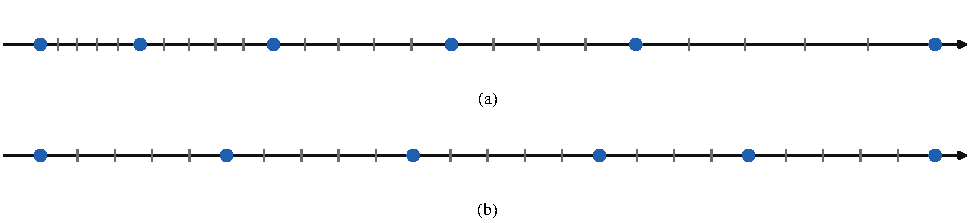
\includegraphics[width=\linewidth]{figures/polsl-osie.pdf}
\sidecaption{Nuty od E2 do E4 (kreski) i sześć strun (niebieskie kropki). (a) Na osi liniowej częstotliwości
odstępy między półtonami rosną: ostatni jest ok.\ 3,8 raza większy niż pierwszy ($2^{23/12}$), więc niskie nuty
tłoczą się przy zerze. (b) Na osi $\log_2 f$ wszystkie półtony są równo oddalone o $1/12$ (z tw.~\ref{tw:log-iloczynu}).
Dlatego model liczy bliskość nut w półtonach, a nie w hercach. \label{rys:polsl-osie}}
\end{figure}

W modelu Gen~6 jedna nuta ma $3$ biny na półton, czyli bin to $100/3\approx33{,}3$ centa. Ewaluacja uznaje
wysokość za poprawną, jeśli różni się od wzorca o mniej niż $50$ centów (ćwierć tonu) --- to ok. półtora biną.

\section{Klatki czasu}

Model nie analizuje całego nagrania naraz, tylko \emph{klatkami}: co $h$ próbek (krok, ang.\ \emph{hop}) bierze okno
długości $N_w$ próbek i liczy z niego widmo (rozdział~\ref{rozdz:fourier}).

\begin{przyklad}[Liczba klatek]\label{prz:klatki}
Gen~6 używa okna $N_w=4096$ próbek ($371{,}5\ms$) i kroku $h=256$ próbek ($23{,}2\ms$). Okno mieści się w nagraniu
o $N$ próbkach dla $t=0,\dots,\lfloor(N-N_w)/h\rfloor$, więc
$T=\lfloor(N-N_w)/h\rfloor+1$. Dla $N=66\,150$ ($6$~s): $T=\lfloor 62\,054/256\rfloor+1=242+1=243$ klatki.
\end{przyklad}

\begin{sprawdz}
\begin{enumerate}
\item Oblicz częstotliwość nuty $m=52$ (E3) i nuty $m=76$. Ile półtonów i ile centów dzieli E3 od E2?
\item Nuta ma częstotliwość $f_1=200\Hz$, a druga $f_2=206\Hz$. Ile centów je dzieli? Czy mieści się w tolerancji $50$ centów?
\item Sinusoida $7000\Hz$ jest próbkowana przy $f_s=11\,025\Hz$. Jaką częstotliwość zobaczy komputer? Skorzystaj z tw.~\ref{tw:aliasing}.
\item Nagranie ma $N=11\,025\cdot 30$ próbek. Ile klatek $T$ daje okno 4096 z krokiem 256?
\end{enumerate}
\end{sprawdz}

\subsection*{Rozwiązania}
\begin{enumerate}
\item $f(52)=440\cdot2^{-17/12}=164{,}81\Hz$ oraz $f(76)=440\cdot 2^{7/12}=659{,}26\Hz$. E3 jest $12$ półtonów, czyli $1200$ centów, nad E2 (stosunek $164{,}81/82{,}41=2$).
\item $c=1200\log_2(206/200)=1200\cdot0{,}0426=51{,}2$ centa, czyli o włos powyżej tolerancji $50$.
\item $f_s-7000=4025\Hz$ (z drugiej części twierdzenia; znak jest przeciwny). Komputer zobaczy ton $4025\Hz$ w przeciwnej fazie.
\item $N=330\,750$ i $(330\,750-4096)/256=1275{,}99\ldots$, więc $T=1275+1=1276$ klatek.
\end{enumerate}
